\documentclass{standalone}

\usepackage{tikz}
\usepackage{bm}
    
\usepackage{graphicx} % Работа с графикой \includegraphics{}
\graphicspath{{./images/img1/}} % картинки в папке ./images/img1/
    
\begin{document}

\begin{tikzpicture}
    \node at(-6.3,0) 
        {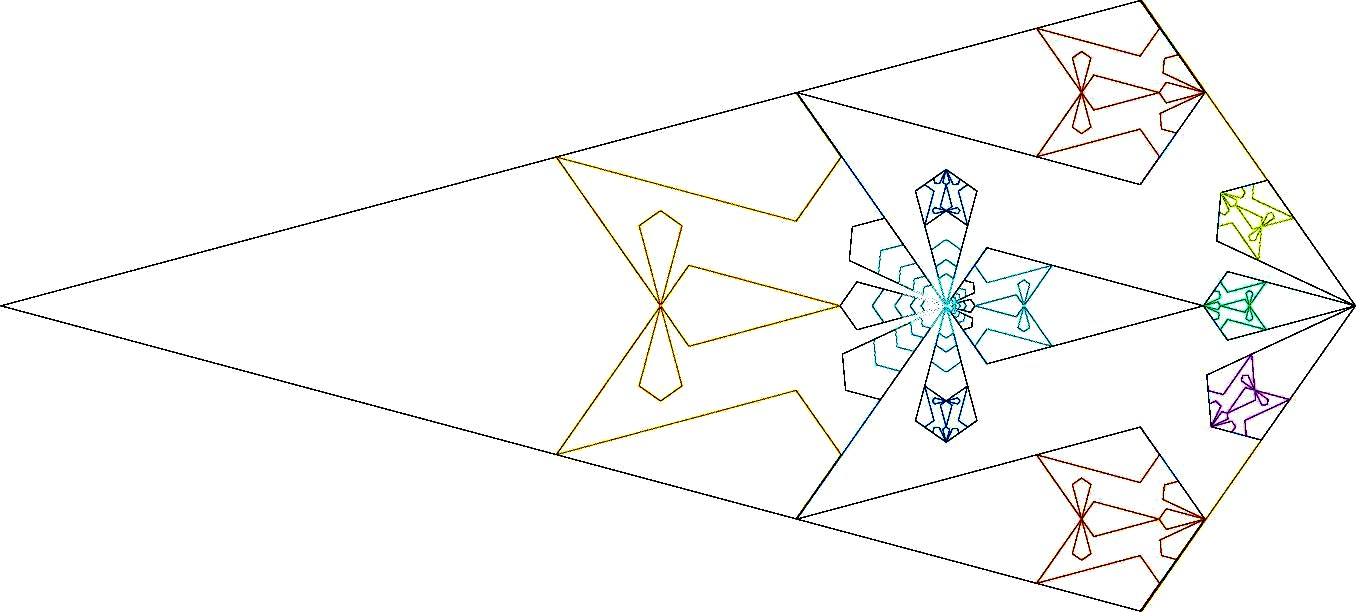
\includegraphics[width=11.9cm]{Pol2a.jpg}};
    \node at(2,0) 
        {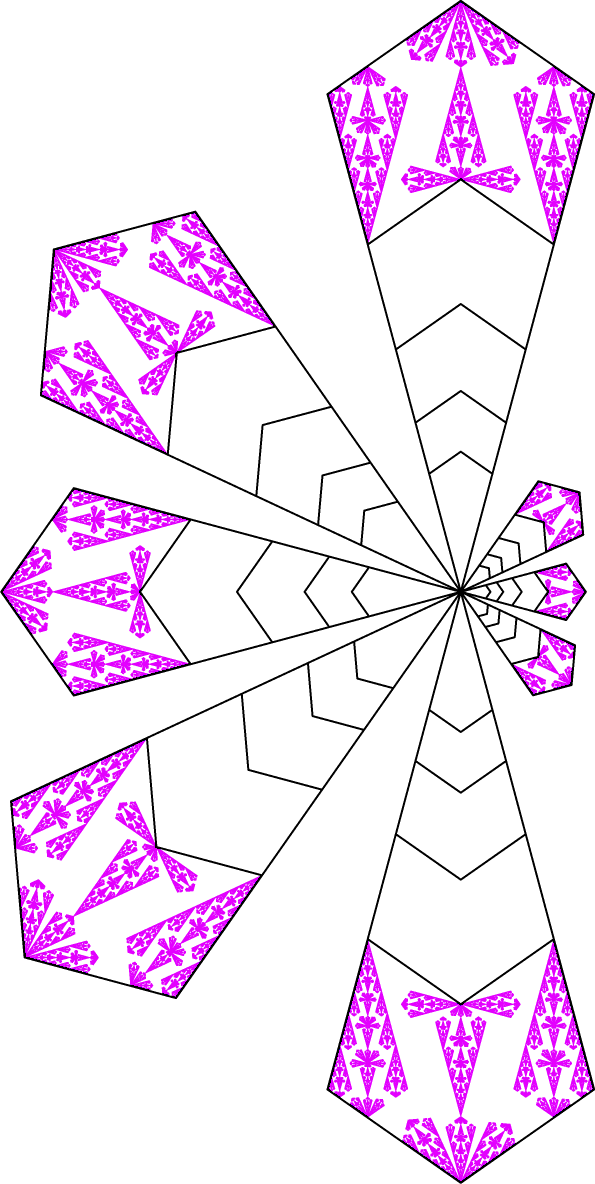
\includegraphics[width=3.4cm]{CU.png}};
    % \draw[step=.1,lightgray,ultra thin] (-12,-4)grid (4,4);
    % \draw[step=1,green,thin] (-12,-4)grid(4,4);
    \draw[thick,blue] (-3.94,0)circle(0.15);
    \draw[thick,red]  (-3.94,0)circle(1.2);
    \draw[thick,blue] (2.95,0)circle(0.4);
    \draw[thick,red] 
        (2.95,3.4) arc (90:150:3.4) 
        (2.95,3.4) arc (90:70:3.4)
        (2.95,-3.4) arc (-90:-150:3.4) 
        (2.95,-3.4) arc (-90:-70:3.4);
    \path[thick,red] (2.95,0) edge[->]  (1.5,3.05);
    \path[thick,blue] (2.95,0) edge[->]  (2.65,-0.3);
    \path[thick,red] (-3.94,-1.2) edge[<->]  (-3.84,-1.5);
    \draw[thick,red] 
        (-0.35,0)--(-2.2,-0.85) 
        (-0.35,0)--(-2.3,-0.5);
    \path[thick,red] 
        (-2.1,-0.45)edge[bend right=10](-2,-0.75);
    \node at(1.5,2.5){$\bm\rho_2$}; 
    \node at(2.5,-0.5){$\bm\rho_1$};
    \node at(-2.4,-0.7){$\bm\alpha_0$};
    \node at(-4.2,-1.4){$\bm\rho_0$};
    % \node at(1.5,-2.2){$\bm\rho_1$};\node at(-2.8,-2.5){$\bm\al_0$};
\end{tikzpicture}

\end{document}